\chapter{Aktueller Entwicklungsstand}

Dieses Kapitel soll einen Überblick über derzeitige Projekte schaffen, die es sich zur Aufgabe gemacht haben, autonomes Fahren weltweit auf die Straßen zu bringen.

\section{Waymo}

Waymo ist ein Schwesterunternehmen von Google und führt das im Jahr 2009 gegründete \textit{Google Driverless Car}-Projekt fort. 2015 fand die erste, voll autonome Fahrt auf öffentlichen Straßen in Austin statt. Im Oktober 2018 erreichte Waymo den Meilenstein von 10 Millionen zurückgelegten Meilen (ca. 16 Millionen Kilometer) in ihrer Flotte von autonomen Fahrzeugen.

Am 5.\ Dezember 2018 startete Waymo ein kommerzielles Taxi-Service namens \textit{Waymo One} in vier Vororten von Phoenix, Arizona. Die autonomen Fahrzeuge werden derzeit noch von einem \enq{Sicherheitsfahrer} begleitet, der im Fall einer Fehlfunktion der autonomen Systeme, die Kontrolle über das Fahrzeug übernehmen kann.
\vgls{waymo-taxiservice} Bereits seit 2017 bis zum Start von \textit{Waymo One} lief das sogenannte \textit{Early rider program}, an dem ausgewählte Bewohner des Ballungsraums von Phoenix teilnehmen konnten, um kostenlose Taxifahrten zu erhalten. Das Feedback der Teilnehmer trug zur Weiterentwicklung der autonomen Fahrzeuge bei.
\vgl{waymo-website}


\section{Tesla}

Tesla ist, ebenso wie Waymo, ein im Silicon Valley ansässiges Unternehmen mit folgendem selbst ernannten Ziel: \zit{tesla-about}{Die Beschleunigung des Übergangs zu nachhaltiger Energie.} Um dieses Ziel erreichen zu können, stellte Tesla im Jahr 2008 den \enq{Roadster} vor, einen zweisitzigen Sportwagen, der die Finanzierung der Premium-Limousine \enq{Model S} sicherte. Besondere Merkmale sind die größte Reichweite unter Elektrofahrzeugen und eine Beschleunigung von 0 auf 100 \si[per-mode=symbol]{\kilo\metre\per\hour} in 2,7 Sekunden. Derzeit läuft die Auslieferung der im Vergeleich zum \enq{Model S} kompakteren Limousine \enq{Model 3}, welches durch einen Grundpreis von 35.000 US-Dollar die Verbreitung von Elektrofahrzeugen weiter vorantreiben soll.
\vgl{tesla-about}

Teslas Fahrzeuge zählen außerdem zu den sichersten der Welt. Wie in \ref{safety-chart} zu sehen, sind von allen seit 2011 von der \ac{NHTSA} getesteten Fahrzeuge, die drei mit der niedrigsten Wahrscheinlichkeit von Verletzungen, alle von Tesla hergestellt. Das \enq{Model 3} hat hierbei einen besonders niedrigen Wert von nur 5,7 Prozent. Dieser Wert errechnet sich durch den \enq{Vehicle Safety Score} von 0,38 der mit der von der \ac{NHTSA} angegebenen Basiswahrscheinlichkeit von 15 Prozent multipliziert wird. \vgls[40038]{nhtsa-baseline}{model-3-score}

\begin{figure}\centering
  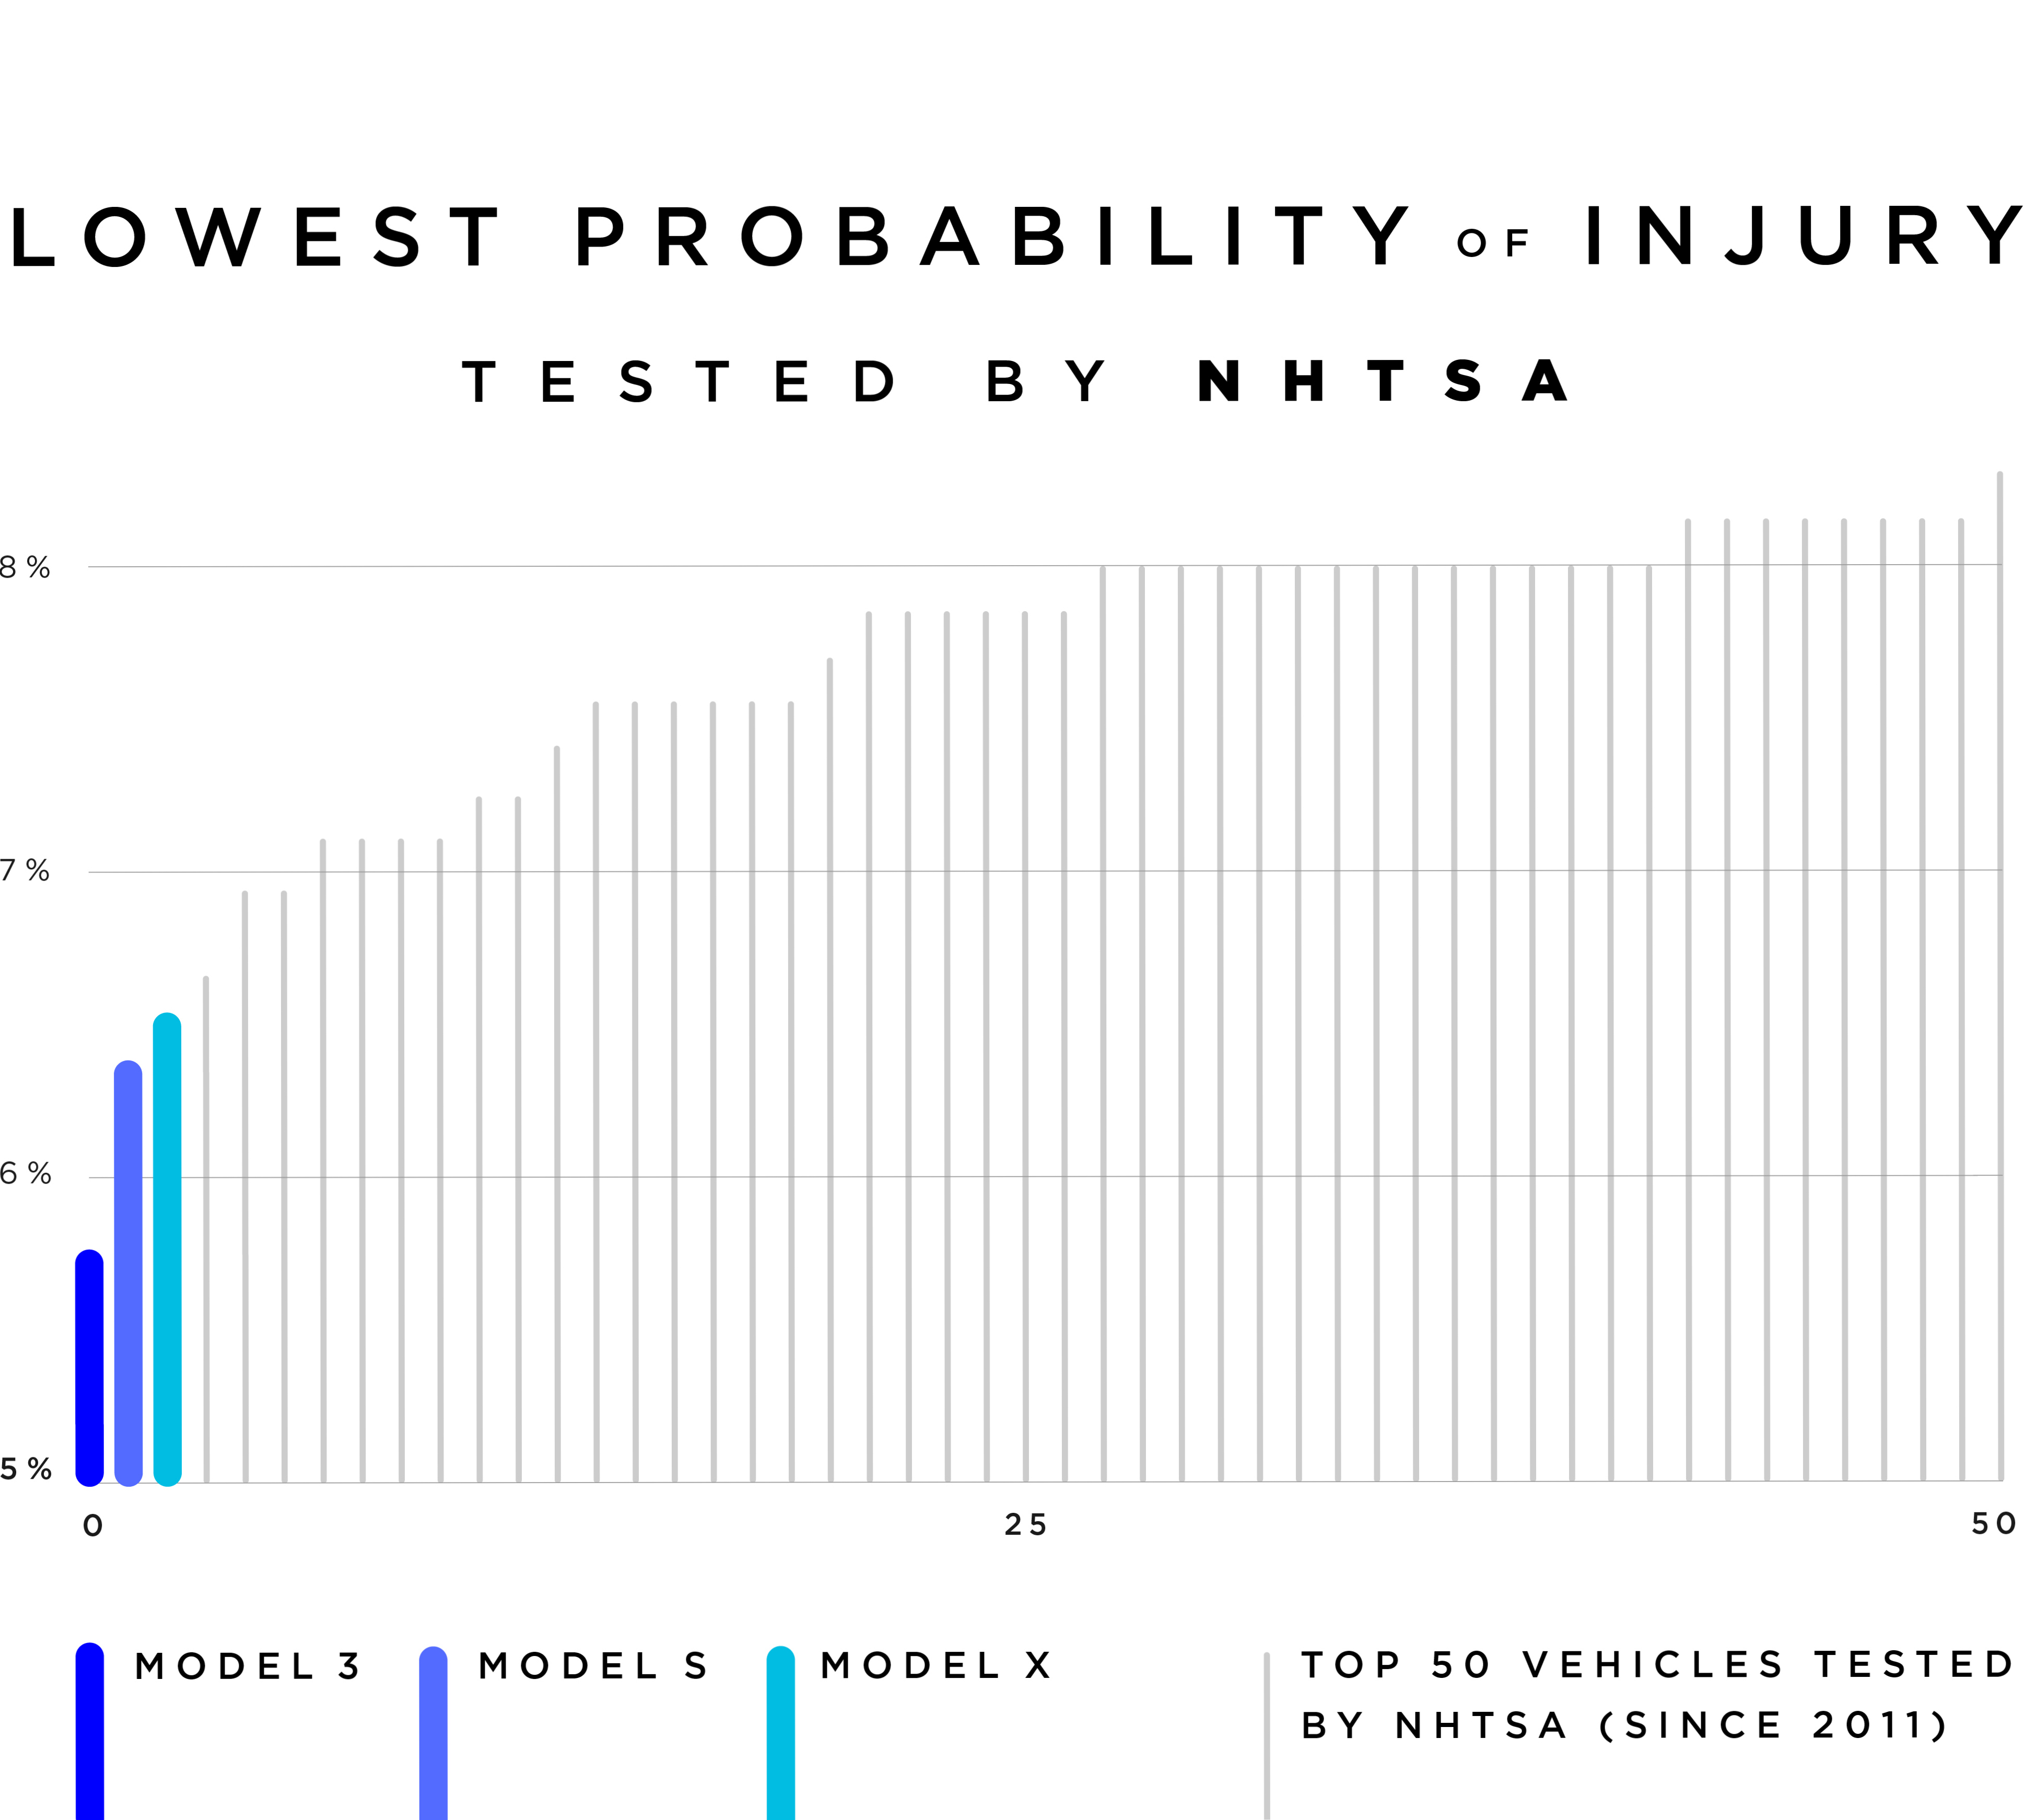
\includegraphics[width=\textwidth]{safety-chart.jpg}
  \captionbelow[Niedrigste Wahrscheinlichkeit von Verletzungen. Getestet von der \ac{NHTSA}. Bildquelle: \fullcite{tesla-safety}]{Niedrigste Wahrscheinlichkeit von Verletzungen. Getestet von der \ac{NHTSA} (\cite{tesla-safety})}
  \label{safety-chart}
\end{figure}

Weiters ist Tesla für seinen bereits in \ref{section-2-3} behandelten \textit{Autopilot}. Am 27.\ November haben Teslas Fahrzeuge eine Milliarde Meilen (ca. 1,6 Milliarden Kilometer) mit aktiviertem \textit{Autopilot} zurückgelegt. Das entspricht etwa 10 Prozent aller von Teslas Fahrzeuges weltweit gefahrenen Meilen, wobei hierbei auch Fahrzeuge ohne \textit{Autopilot}-Hardware bzw. solche mit Hardware, jedoch ohne der notwendigen kostenpflichtigen Aktivierung des Assistenzsystems miteingerechnet werden. \vgl{electrek-one-billion}


\section{Wiener Linien}

Im Frühjahr 2019 soll die erste autonome Buslinie Wiens in der Seestadt in Betrieb gehen. Das Projekt namens \textit{auto.Bus - Seestadt} durchläuft derzeit intensive Testfahrten auf geschlossenem Gelände. Bei dem Bus handelt es sich um einen vollelektrischen Kleinbus (siehe \ref{bus-seestadt}), der Platz für bis zu zehn Fahrgäste und einen Operator bietet. Der Operator ist derzeit noch aus sicherheitsgründen notwendig, er überwacht den Bus und kann im Ernstfall ins Geschehen eingreifen. \vgl{wiener-linien}

\begin{figure}\centering
  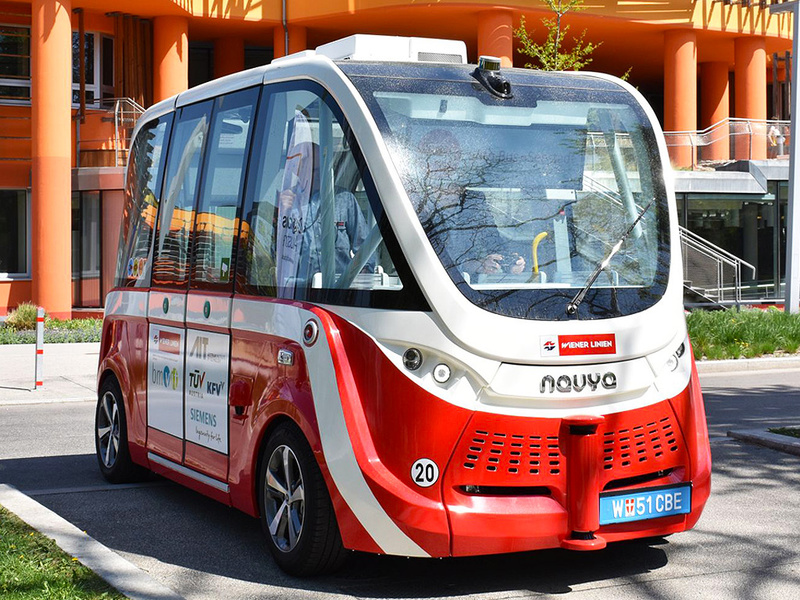
\includegraphics[width=\textwidth]{bus-seestadt.jpg}
  \captionbelow[Elektrischer Kleinbus der Wiener Linien. Bildquelle: \fullcite{wiener-linien}]{Elektrischer Kleinbus der Wiener Linien (\cite{wiener-linien})}
  \label{bus-seestadt}

  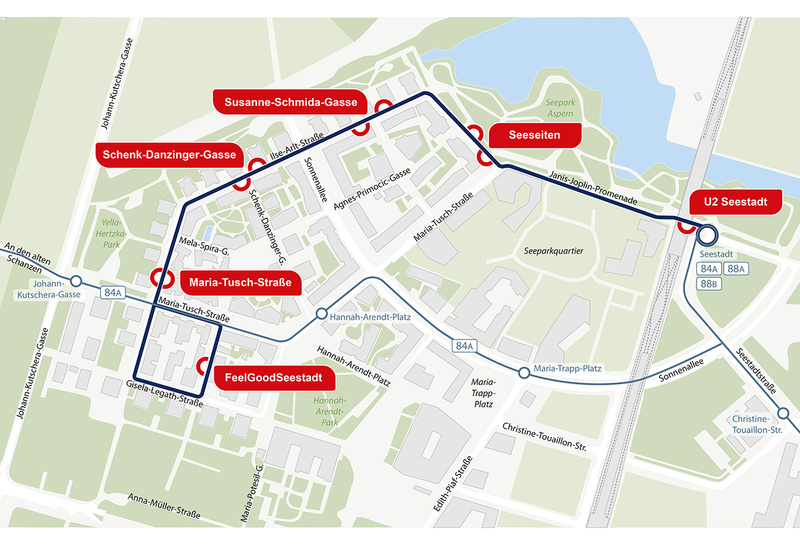
\includegraphics[width=\textwidth]{bus-seestadt-karte.jpg}
  \captionbelow[Geplante Route der autonomen Buslinie. Bildquelle: \fullcite{wiener-linien}]{Geplante Route der autonomen Buslinie (\cite{wiener-linien})}
  \label{bus-seestadt-karte}
\end{figure}

Die geplante Route ist in \ref{bus-seestadt-karte} dargestellt, sie ist 2 \si{\kilo\metre} lang und bedient sechs Stationen in der Seestadt. Die Beförderung auf der Linie ist kostenlos. Da es sich um einen Testbetrieb handelt, ist der Transport von Kinderwägen und Rollstühlen rechtlich nicht erlaubt.
\vgl{wiener-linien}


\section{Aktionspaket des Bundesministeriums}

some text
\vgl{bmvit}

some more text
\vgl{bmvit}
